
\documentclass{kuisthesis}


\usepackage{float}
\usepackage{color}
\usepackage{multicol}
\usepackage[dvipdfmx]{pict2e}
\usepackage{graphicx}
\usepackage{ulem}
\usepackage{amsmath,amssymb}
\usepackage{wrapfig}

\jtitle[警備員ロボットの抑止力向上のためのオペレータ支援システム\\に関する研究]{警備員ロボットの抑止力向上のための\\オペレータ支援システムに関する研究}
\etitle{Study on Operator Support System for Improving Deterrence of Security Robot}
\jauthor{天野 岳洋}

\eauthor{Takehiro Amano}
\supervisor{神田 崇行}
\date{2024年1月31日}
\begin{document}
\maketitle
%=====================================================================================

\begin{jabstract}


アバターロボットが普及しアバターを介して遠隔地から勤務することが新たな働き方として認められつつある。
アバターロボットは従来のミーティングアプリを用いたリモートワークでは難しかった物理的作業を伴う
業務であってもリモートワークが可能なことが大きなメリットであり、
リモートワークは通勤の必要がないことや、ワークライフバランスの向上などの様々な面で優れている。
そのためアバターロボットを介した勤務は今後ますます普及することが予想される。
また様々な業務の中で重要とされる注意という行為において
ロボットを介して行うことで、注意した相手とのトラブルを避けることができることも長所としてあげられる。

しかし、ロボットによる注意には大きな問題点もある。
それは注意するために必要な操作が難しいことと、注意したときに相手にその行動をやめさせる力、抑止力が欠如しているというものである。
そこで本研究ではオペレータの支援を行うシステムの開発を行うことでこれらの問題を解決することを目指す。
また研究と実験を進めるにあたって、アバターロボットを用いた警備員業務の中で歩きスマホを注意するシチュエーションを考えた。

%予備実験 理由の順番

ロボットの歩行速度や人との画面上で遠近感をつかみづらいなどの理由から、
アバターロボットを用いた注意に求められる移動操作が困難であった。
したがってまずオペレータ支援のために移動支援システムの開発を行った。
これによってオペレータはカメラ映像上で歩きスマホをしている人の指定を行うだけでよく、システムが
移動先の予測や、それに基づいた人の距離を保った移動、ロボットの向きの調整を担う。
%もう少し難しさをアピールできたら <- OK

%抑止力の向上のために注意文言に注目して、 <- OK
次に有効な注意文言を推薦する発話支援システムによって次に抑止力の欠如を解決できると考えた。
なぜならオペレータが有効な注意文言をとっさに考え付くことが難しいために、抑止力の欠如が生じていると考えられるからである。
この発話支援システムは、状況に応じた有効な注意文言と状況の判断を行うモデルを作成し、それらを用いてオペレータに推薦を行うことによって作成できる。

そこでまず有効な注意文言に関して認知的不協和理論に基づいて検討する。
ここで認知的不協和理論を用いた理由は、注意されても行動をやめない理由が説明可能になるからである。
具体的に注意されたことで「歩きスマホは危険である」という信条と、「自分は歩きスマホをしている」という行動に関する認知とが矛盾することに気づかされ、
その認知の矛盾によって不快感が生じ、その不快感の解消のために行動をやめる。
しかしこの時行動をやめる以外にもこの不快感を解消できるため、これを注意されても歩きスマホをやめない人がいることの説明とできる。
そこでとられた解消方法に対抗するような文言によって、不快感の解消を困難にし行動をやめるように誘導するできると考えられる。
こうして有効と考えられる注意文言がとられた解消方法ごとに得られた。

次にそれらの不快感の解消方法に基づく注意文言の推薦にあたり、解消方法を推定するモデルの構築のために実験を行った。
解消方法の推定には認知的不協和理論についての知識や相手の行動に対する洞察が必要であり、
解消方法の推定をオペレータが行うことは難しいため、解消方法の推定を行うモデルが必要となる。

実験では事前に協力をお願いした2人の参加者に対して注意されたときにどのように感じたかのアンケートを、
また歩きスマホをしていた5組のATCへの来客者に対して注意を行ったときの反応の観察を行なった。アンケートでは
一部の注意文言が使用された際に、自分だけが注意されているという孤立感から周囲の圧力を感じることで無視することが難しくなった
という意見が得られた。また実際の観察では、歩行速度やグループの人数といった属性の値によって解消方法を推定することができる可能性が示唆された。

以上のように本研究では移動操作の支援を行うシステムの開発を行い、また抑止力向上のための発話支援システムの開発に取り組んだ。
発話支援システムの開発のためには、今後不快感の解消方法を推定するモデルの構築が必要であるが、
実験の観察からいくつかの値から解消方法の推定が行える可能性が示唆された。またアンケートの結果からは、
同調圧力に基づいた戦略を取り入れたシステムの構築も考えられる。
%可能性がある。 できるようになる <- OK
\end{jabstract}


\begin{eabstract}
With the spread of avatar robots, working remotely via avatar is 
gaining recognition as a new way of working. The major advantage of 
avatar robots is that they enable remote work even for tasks that require 
physical work, which has been difficult with such conventional remote work as using
meeting applications. 
Therefore, it is expected that work via Avatar robots 
will become increasingly popular in the future. In addition, one of the advantages of using avatar robots is that
it is possible to avoid trouble with the person who is admonished through
the robot.

However, there are some problems with admonishing through the robot.
One is the difficulty of moving the robot required to
admonishing, and the other is the lack of deterrence when admonishing.
Therefore, in this study, we aim to solve these problems by developing a system to support operators.
In addition, in order to conduct research and experiments, we considered a situation where a security 
robot as avatar admonishes a person who is walking while using a smartphone.

The speed of the robot's walking and the difficulty of grasping the sense of distance
on the screen made it difficult to move the robot required for admonishing.
Hence, we first developed a movement support system for operator support.
With this system, the operator only needs to specify the person who is walking while using a smartphone
on the camera image, and the system will predict the destination, move while maintaining the distance from the person,
and adjust the orientation of the robot.

Next, we considered that lack of deterrence could be solved by creating a speech support system that recommends effective admonishing words.
This is because it is difficult to come up with effective admonishing words on the spot, which is considered to be the cause of the lack of deterrence.
This speech support system can be developed by listing effective words according to situations, creating a model that makes judgments about situations 
and recommending effective words according to the judged situation.

Therefore, first, we considered effective admonishing words based on cognitive dissonance theory.
The reason for using the theory is that it can explain why people do not stop walking while using a smartphone even if they are admonished.
Specifically, when admonished, people realize that their cognitions are contradictory, 
and they feel uncomfortable due to the contradiction in their cognition.
However, this discomfort can be resolved not only by stopping the behavior, but also by other means, 
so it can be explained why some people do not stop walking while using a smartphone.
Thus, the admonitory words that prevent the discomfort from being resolved should induce the person to stop walking while using a smartphone.

Next, in order to recommend admonishing words based on these methods of resolving discomfort, 
we conducted an experiment to construct a model for estimating it.
Estimating it requires knowledge of cognitive dissonance theory 
and insight into the other person's behavior, so it is difficult for the operator, and a model is needed.

In the experiment, we conducted a questionnaire on how two participants who had been asked for cooperation felt 
when they were admonished, and observed the reactions of five pairs of visitors when they were admonished.
In the questionnaire, it was found that in some cases,
it was difficult to ignore them because of the feeling of isolation and the feeling of pressure from the surroundings. 
In the actual observation, it was suggested that the method of resolving 
discomfort could be estimated depending on the values such as walking speed 
and the number of people in the group.

Thus, in this study, we developed a system to support the movement operation and a speech support system to improve the deterrence.
In order to develop the speech support system, it is necessary to construct a model that estimates the method of resolving discomfort in the future, 
but it was suggested from the observation of the experiment that it could be estimated from some values. In addition, from the results of the questionnaire, it is also possible to construct a system that incorporates a strategy based on conformity pressure.

\end{eabstract}
%=====================================================================================

% 目次の表示
\tableofcontents


%=====================================================================================
%=====================================================================================

\section{はじめに} %章
\label{sec: はじめに} %節
%アバターロボットについての説明
近年、アバターロボットを用いた遠隔業務が注目されている。
アバターロボットとは人間が遠隔地からロボットを操作することで、
人が実際にその場所に行くことなく現地での作業を可能にするロボットのことであり、
%memo 違和感感じる?? 保留
そのロボットを介して遠隔地から作業を行うことをテレオペレーションと呼ぶ。

アバターロボットを用いることの大きなメリットは、その性質から
それまで難しかった物理的な作業を伴うサービス業や飲食業などの分野におけるリモートワークを可能にすることである。
例えばugo株式会社\footnote{https://ugo.plus/}によるアバターロボットugoは、
ビルメンテナンスや警備業務のためのアバターロボットであり、
トイレ清掃や警備、巡回等の業務を遠隔地から行うことができる。
リモートワークの長所として、働く場所を問わないことから通勤の必要がないことや、ワークライフバランスの向上、
時差を利用した業務が可能になることなどがあげられる。
加えて他の人間と直接接する機会が少ないことなどから、
パンデミック時において感染を心配する必要がないことも大きなメリットである。
実際にアメリカでは2020年の新型コロナウイルスの流行によって、
それまでは従業員のうちリモートワークをしている割合は約13\%だったが、
2020年の4月にはおよそ56\% $\sim$ 74\%に増加した\cite{ozimek2020future}。
またリモートワークは従業員だけでなく企業にとっても利点があることがわかっている。
例えば\cite{FERREIRA202170}では、企業が地理的制約なしに優秀な人材を獲得できることや、
オフィスの維持費や交通費を削減できることがあげられている。

%その他のアバターロボットのメリットとしては、身体障碍を持つ人が
%身体労働をともなう業務に従事することを可能にすることがあげられる。
%さらにその際に、身体障碍を持つ人の社会参加感や精神的充足感をもたらすことがわかっている\cite{takeuchi2020avatar}。
またアバターロボットは自律ロボットでは難しかった人との柔軟なコミュニケーションが可能である。
現時点で自律ロボットは人の表情や声のトーン、仕草などを読み取り相手の感情を推測することが困難であることや、
音声認識の問題などから人とのコミュニケーションにおいて限界があるが、
一方でアバターロボットでは人が操作するため、人とのコミュニケーションにおいて自律ロボットよりも柔軟な対応が可能である。
これから更なる通信技術の向上、安価なロボットの流通に伴いアバターロボットを介した業務はますます普及することが予想される。

今後アバターロボットが担うであろう様々な業務において人々を注意し、
特定の行動を抑止するという行為は重要である。
例えば、教育の場面において先生は生徒が集中力に欠く行動をとっていたとき、
注意することによってその行動をやめさせ生徒の集中を取り戻すことができる。
またサービス業の場面においては、
他の客に迷惑をかける行動を取る客がいたときに店員が注意することで、
その行動をやめさせ他の客の満足度の低下を防ぐことができる。
しかし、人を注意するという行為には逆上した注意相手とのトラブルに陥るかもしれないといったリスクも伴う。
ロボットを用いた場合、注意相手との直接のコミュニケーションが存在せずそのようなリスクが小さいことから、
ロボットは注意を行う際の便利なツールとなる。
以上のことから、注意が重要となる業務の中でアバターロボットは重要な役割を果たすことになる。

しかしロボットによる注意には問題点もある。
それは注意のために求められる移動操作の困難性と抑止力の欠如である。
ここで本研究では「抑止力」を歩きスマホのような社会的規範に背くような行動をしている相手に対して
注意を行ったときに、その行動をやめさせる力と定義する。

移動操作に関して、
ロボットの最大移動速度は安全のために通常の人の歩行速度より低めに設定されていることや、
ロボットからのカメラ映像では空間認識が困難であることから、
移動操作が難しくそもそもその人の視界に入ることが難しい場合がある。
抑止力に関して例えば\cite{Schneider2022}では、歩きスマホをしている人に対してロボットが2回にわたって
「歩きスマホ危険ですからおやめください」と注意を行った時に、
160人中76人が1回目の注意を無視し、さらにそのうち72人が2回目の注意も無視したという結果が得られている。
同論文では1回目の注意を無視した人に対して、「あなたはただのロボットだとお思いみたいですが、私はみんなのために働いているのですよ」
と注意することによって無視する人が有意に減少したという結果も得られているが、
オペレータがとっさにそのような効果的な注意文言を考えることは難しい。

アバターロボットを介した業務の普及が予測される中で、
注意時における移動操作の困難性と抑止力の欠如の解決が求められる。そこで本研究では
これら二つの課題に取り組む。移動操作の困難性の解決のために移動支援システムの開発と、
また抑止力の欠如の解決のために\ref{sec: CDT}章で説明する認知的不協和理論\cite{Festinger1957}に基づいた有効な注意文言の推薦システムの開発を目指す。
これは規範に反する行動を注意されてもその行動をやめない人がいる理由を認知的不協和理論によって説明可能であるからである。
具体的には、まず注意されることによって自らの信条と自らの行動に関する認知とが矛盾することに気づかされ、
認知の矛盾によって不快感がうまれる。
そしてその不快感の解消のために注意された行動をやめる。
しかしこの不快感の解消は行動をやめること以外によっても可能であるため、
これを注意をされても行動をやめない人がいることの説明とできる。
\section{関連研究}
このセクションでは移動支援システムを設計する上でロボットの接近行動に関する研究について、また
注意文言の検討に用いた認知的不協和理論をHuman-Robot Interaction(HRI)分野に適用した研究について
紹介を行う。さらに歩きスマホを注意しやめさせるといった、人の行動に影響を与えるた
めに否定的なフィードバックや行動をとるロボットに関する研究についてそして
注意文言提示システムのようなテレオペレーション支援に関する研究について様々な例と本研究との差
異について説明を行う。
\subsection{ロボットの接近行動に関する研究}
ロボットを人間の近くに移動させることは人間とコミュニケーションをとるうえで重要な行為であり、
この行為に関する研究は多く存在するが、多くは自律ロボットを前提としたもので
オペレータの存在を想定していない。

例えば\cite{woods2006methodological}では、
机の前に座っている人には後ろからや真正面から近づくよりも、斜め前から近づくほうが人にとって快適であることなどが示されている。
また\cite{joosse2021making}ではロボットが人に十分に近づく際に、接近速度が速い(1.0m/s)ほうが、
遅い(0.4m/s)ときに比べて、人のポジティブな反応(e.g., 笑顔を見せるや寄りかかるといった行動)が見られることが示されている。
また\cite{satake2009approach}では人の過去の行動から人の経路予測やその人の意図を用い、
ロボットが周囲の人々の中でもっとも話しかけやすい人への移動を行うようなアプローチ方法によって
最も近い人に最短距離で近づくよりも、無視される、気づかれないといったことなく会話を始めれることが示されている。
他にも最短距離で近づくよりも、途中で角度を変えて人に急接近するような近づき方によって、
ロボットの抑止力が上がることが示されている\cite{Mizumaru2019}。


しかしこれらのように多くの研究では、自律ロボットを前提としておりある特定の人への近づき方に
ついて研究を行っており、近づく人の選択はできないもしくは考慮されていない。\cite{Mizumaru2019}では
近づくべき人が選択できるようになっているが、それはあくまでWizard of Oz手法の中で用いられているものでありインターフェースなどは
作成されていない。そこで本研究ではアバターロボットを操作する際に、近づけるか否かや視野外に人がいるか等の情報をインターフェースを介してオペレータに提供することによって
、オペレータが近づける人の中で自由に接近対象を選べるようにし、その後適切な方法で近づくことを可能にするシステムの開発を行う。

\subsection{認知的不協和のHRIへの適用研究}
%認知的不協和理論の説明ここで行う
認知的不協和理論\cite{Festinger1957}は、現代においてもマーケティングや心理学など幅広い分野で用いられている理論であり
HRI分野における適用例も多いが、それらのほとんどは結果の説明に用いているのみである。

例えば研究\cite{washburn2022exploring}では、
人間が荷物配達ロボットに対して従順になる理由の説明として、認知的不協和理論を用いている。具体的には、
人間がロボットにタスクを依頼された場合に、人間が「タスクを果たすことを楽しいことだ」という認知を追加する傾向があることを
人間がロボットに対して従順になりやすいことの説明としている。また他にも研究\cite{herse2018you}では、ロボットがわざと
最適ではない選択肢を人間に提供した際に、信頼されているロボットのほうがそうでないほうよりも、人間が反応を返すまでに
長い時間がかかることが示されている。この理由として
人間がロボットを信頼している場合ロボットが不適切な選択肢を提示した際に、
不協和が生じ意思決定時に余分な負荷がかかるために、反応時間が長くなるという説明を行っている。
これらのように多くの研究は、
あくまで結果の説明のために認知的不協和理論を用いているものであり、
ロボットがとるべき戦略を決定するために用いているものではない。

認知的不協和に基づく不快感を戦略として利用した歩きスマホの注意を行っている研究\cite{Schneider2022}は存在しているが、
一部分のみの利用にとどまっている。具体的に上記研究では自律ロボットを前提としているため注意された時に生じる不快感の解消方法として、
いずれが用いられているかのその場での分別は難しいものとしており、行動をやめるか、ロボットの矮小化を行うことを仮定している。これは
注意を無視した人のアンケートで、歩きスマホを行っている人が注意された際に用いる「行動を変える」以外の不快感の解消方法として、
ロボットの矮小化が多かったためである。ロボットの矮小化とは例えば、
ロボットが機械音声を用いているために、ただのガイダンスだと捉えられたや、ロボットがただの機械であると捉えられたなどである。
そのため、一度単に「歩きスマホは危険なのでおやめください。」と注意されたが引き続き歩きスマホを行っている人に対して、
「あなたは私のことをただのロボットだと思っているかもしれませんが、私はみなさんのために働いているのです」と一律に話しかけることによって、ロボットの矮小化
を防ぐことを試みている。一方で本研究ではアバターロボットを用いており、オペレータとして人間が操作することを前提としているため、
より幅広い戦略をとることが可能である。そこで、使用されたであろう解消方法に基づいた注意を行うことでより効果的な注意を行うことができるのではないかと考える。

\subsection{説得のために否定的な行動をとるロボット}

ロボットがいかにして人間に対する説得力を向上させることができるかについては多くの先行研究で取り組まれているが、
なぜ説得がうまくいかないかに基づいて戦略を決定しているような研究は少ない。
ここで説得は人の行動になにかしらの影響を与えるために行われるものであり、
本研究で取り組む抑止は特にその中でも、
特定の行動をやめさせるための説得行為を指すものとする。

例えばロボットが人間とのじゃんけんゲーム内でわざと負けることによって贈賄を行い、
その後人間がロボットにお願いされた追加のタスクを行うかどうかについての研究\cite{sandoval2016can}では、
ロボットがわざと負けた場合に(贈賄を行った場合)より好感度が高く、
しかし、追加のタスクについてはより非協力的になることがわかっている。また、他にも仮想的な洗濯作業中に省エネを促す際、エネルギーをより使う設定に変えた際に、怒りの表情や批判的な言葉または不快な音といった否定的なフィードバックをとるほうが、
エネルギーを節約する設定に変えたときに、褒めるや喜びの表情を見せるといった肯定的なフィードバックよりもより効果的に人間に行動の変容をもたらすことがわかっている\cite{Midden2009}。
また研究\cite{paradeda2019makes}では、被験者が自律ロボットから助言を受けながら決断を下すようなシチュエーションにおいて、ロボットが怒り等の負の感情を
表現すると、被験者はロボットのアドバイスに従う可能性が高くなり、説得が効果的になることが報告されている。しかし、
一般的にどのようなフィードバックが最も説得力があるかという研究課題に対する明確な答えはなく、それは実験のシチュエーションや人間と
ロボットの関係性によって異なる。そこで本研究では、規範に反する行動を注意されてもやめない理由を考察したうえで、
どのような注意がその行動をやめさせるのに効果的であるか研究する。
\subsection{テレオペレーション支援に関する研究}
テレオペレーション支援に関する研究は多く行われており様々な面から種々のシステムが開発されてきたが、
オペレータは依然としてその場において効果的な操作内容や発言内容を自ら考えなければならずその負担は大きい。
例えば\cite{chen2007human,triantafyllidis2020study}では、テレオペレーションにおいて課題となっている視野の狭さや方向感覚の喪失といった問題を、
視覚だけでなく聴覚や触覚などの他の感覚を利用する多モーダルインターフェースによって解決を試みている。
また、多数の無人航空機を操作する際にパフォーマンスを向上させる
ようなコントローラーへのハプティックフィードバック手法についての研究\cite{son2011measuring}などがある。
へパティックフィードバックとは、コントローラーの利用者に力や振動によって警告等を行うフィードバック手法のことである。
他にも鉱業において採掘を行うロボットのテレオペレーションでの
ユーザーインターフェースについての研究\cite{hainsworth2001teleoperation}や、
テレオペレーターが荒い言葉遣いで話したとしても意図認識を用いて、支援システムが丁寧な言葉遣いに変換するような支援システム\cite{Daneshmand2023}などいろいろなものが研究されている。
しかし、これらの研究のように大半では操作や発言を行いやすくするための支援に関する研究であり、
それらの操作内容や発言内容は操作者が決定しなければならず、オペレーターは
どういった操作、どういった発言が効果的かを考える必要がある。
そこで本研究では業務の中で必要な知識をオペレータに提示し、
オペレータは
自分でどのようなものが有効か考える必要なく有効な注意喚起を行うことが可能になるような
支援システムの開発を目標とする。


\section{認知的不協和とは} %1.1.2
\label{sec: CDT}
この章では、人が注意されたときに不快感が生じる理由とその不快感の解消のために人がどのような方法をとれるかについて説明のために、
認知的不協和理論について紹介を行う。
認知的不協和理論\cite{Festinger1957}とはFestingerにより提唱された理論であり、人間が互いに相反する認知を抱いた場合、その状態(不協和)に不快感を感じ
その不快感の解消のために、不協和の解決を図るというものである。
この認知とは、行動、知覚、態度、信念、感情といった様々な事象に関するものであり、多くの場合片方の認知は自らの行動に関するものである。

例えば、表\ref{fig: CDTExample}のようにたばこは健康に良くないと分かっているのに、タバコを吸ってしまった際に生じる不快感が認知的不協和である。
この不快感は、認知1と認知2が矛盾しているために生じるものである。
\begin{table}[H]
  \centering\caption{認知的不協和の例}
  \label{fig: CDTExample}

  \begin{tabular}{c|c}
      認知1 & たばこは体に害をもたらす  \\ \hline
      認知2 & 私はたばこを吸っている \\ 
  \end{tabular}
  
\end{table}
この不快感を解消するために、「行動を変える」「認知を変える」「新たな認知の追加を行う」「矛盾の矮小化、無視」の4つの選択肢をとることができる。
それぞれについて表\ref{fig: CDTExample}のたばこの例を用いて具体的に説明を行う。
\begin{enumerate}
  \item 行動を変える \\
  行動を変えることは、たばこを吸うのをやめることであり表\ref{fig: CDTExample}の認知2の変化をもたらす。そして表\ref{fig: ReduceDissonanceAction}のように認知1と認知2の不一致を解消することができる。
行動の変更が容易なものであればこの方法をとることが最も理論的であるが、行動の変更が困難な場合もある。そのような場合
この方法ではなく他の方法をとることになる。
  \begin{table}[H]
    \centering
    \caption{行動を変える例}
    \label{fig: ReduceDissonanceAction}
    \begin{tabular}{c|c}

        認知1 & たばこは体に害をもたらす  \\ \hline
        認知2 & 私はたばこを\sout{吸っている}吸わない \\
    \end{tabular}
\end{table}
 \item 認知を変える \\
  認知を変えることは、表\ref{fig: CDTExample}の認知1を「たばこは体に害をもたらさない」とすることである。
  これにより認知は表\ref{fig: ReduceDissonanceChange}のように変化し、
  実際に行動を改めることなく認知1と認知2の不一致を解消することができる。
  \begin{table}[H]
    \centering
    \caption{認知を変える例}
    \label{fig: ReduceDissonanceChange}
    \begin{tabular}{c|c}
        認知1 & たばこは体に害を\sout{もたらす}もたらさない  \\ \hline
        認知2 & 私はたばこを吸っている \\
    \end{tabular}
    
  \end{table}

  \item 新たな認知の追加 \\
  新たな認知の追加を行うことは表\ref{fig: CDTExample2}の認知3や認知4を追加することであり、
この追加によって認知1と認知2の不一致度合いを軽減させることができるため生じる不快感が小さいものとなる。
\begin{table}[H]
  \centering
  \caption{新たな認知の追加の例}
  \label{fig: CDTExample2}
  \begin{tabular}{c|c}

      認知1 & たばこは体に害をもたらす  \\ \hline
      認知2 & 私はたばこを吸っている \\ \hline
      認知3 & \textbf{喫煙をやめると他の人にあたってしまい迷惑となる} \\ \hline
      認知4 & \textbf{たばこを吸っていて長寿の人もいる} \\ 
  \end{tabular}

\end{table}

  \item 矛盾の矮小化、無視 \\
  矛盾の矮小化、無視では認知自体を変えずに不協和を解消する方法である。このとき、注意してきた対象や
  認知同士が生む不協和が矮小化もしくは無視されることになる。例えば、そもそも表\ref{fig: CDTExample}の認知1と認知2が
それほど矛盾していないと思い込むことによって生じる不快感を軽減することができる。

\end{enumerate}
\vspace{3mm}

ここで本研究では上記方法が一つ取られた時点で、不快感が十分に解消されそれ以上の方法をとることがないことを仮定する。
従って不協和による不快感が生じた人は上記の方法のうちいずれか一つをとることになる。

\section{研究の前提}
本研究で解決すべきは、アバターロボットを用いた注意活動における移動操作の困難性と抑止力の欠如という問題である。
この章では実験と研究を進める上で、定義や想定するシナリオ、用いるロボットについて説明を行う。

\subsection{抑止力の定義}
本研究において「抑止力」を\textbf{社会的規範に背く行動を行っている相手に対して、注意を行った際にその行動をやめさせる力}と定義する。
つまり抑止力の高い注意とは、注意を受けた際にその注意を無視して行動を続けることが難しいようなものである。

\subsection{想定する状況}
実験研究を進めるうえでアバターロボットが注意する状況として警備員業務を想定し、
その中で注意すべき行動を[4,6]と同じように歩きスマホとした。これは、歩きスマホがもっともよく観測
される迷惑行為であり、実際にやめたかどうかを確認することが容易であるためである。

\subsection{ロボット}
\begin{wrapfigure}{l}{0.3\textwidth}
  \centering
  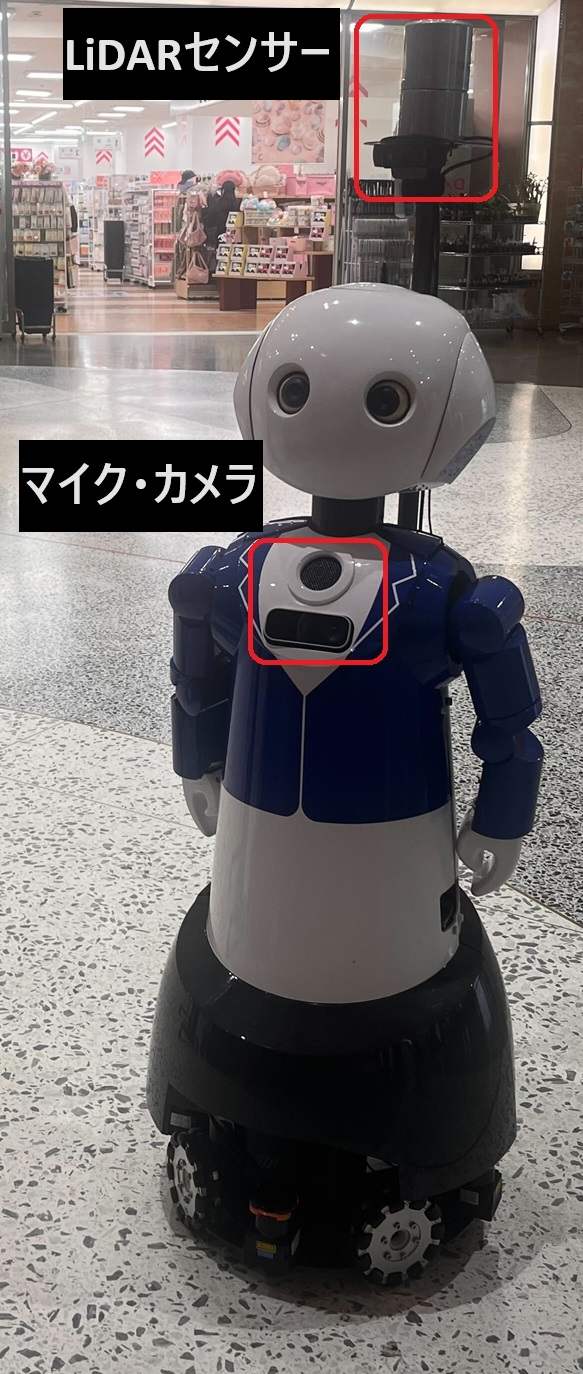
\includegraphics[width=0.25\textwidth]{img/robovie.jpg}
  \caption{Robovie}
  \label{pic:robovie}
\end{wrapfigure}
今回警備員アバターロボットとして用いるロボット「Robovie」の外観を図\ref{pic:robovie}に示す。
Robovieは身長が約120cmであり、4輪の車輪によって前後移動だけでなく左右にも移動することができる。また、
胸部にはカメラとマイクおよびスピーカーが搭載されており、頭上部にはLiDARセンサーが搭載されている。
このLiDARセンサーによりロボットは360度すべての方向の物体を検知することができる。
オペレータはこのロボットからの情報受け取り、ロボットを発声や移動等の命令を行い操作することができる。
なおこれらデータのやり取りはROS\footnote{https://wiki.ros.org/ja}を介して行われる。ROSとは、
ロボットのソフトウェア開発のためのオープンソースソフトウェアであり
ROSを用いることで複数のプロセス間でのデータのやり取りを容易に行うことができる。

\clearpage

\section{提案手法}

アバターロボットを用いた注意活動には注意のための移動操作の困難性と、
抑止力の欠如という二つの課題がある。そこで移動操作の困難性の解決のために移動操作支援システムを作成し、
また抑止力の欠如の解決のために有効な注意文言を提示することでオペレータの発話支援を行うシステムの開発を行う。

\subsection{移動操作支援システム}
移動操作を簡単にするためのシステムの開発を行った。これは、より人間らしい対話のためにオペレータ自身が発話を行う必要がある中で、
ロボットの移動操作が困難性から発話に集中できないといった問題や、そもそも話しかけることができないという問題の解決のためである。

システム全体の構成を図\ref{pic:systemcompose}に、インターフェースを図\ref{pic:interface}に示す。
\begin{figure}[htb]
  \centering
  \includegraphics[width=15cm]{img/system\_compose.drawio.png}
  \caption{移動支援システムの構成}
  \label{pic:systemcompose}
\end{figure}
\begin{figure}[htb]
  \centering
  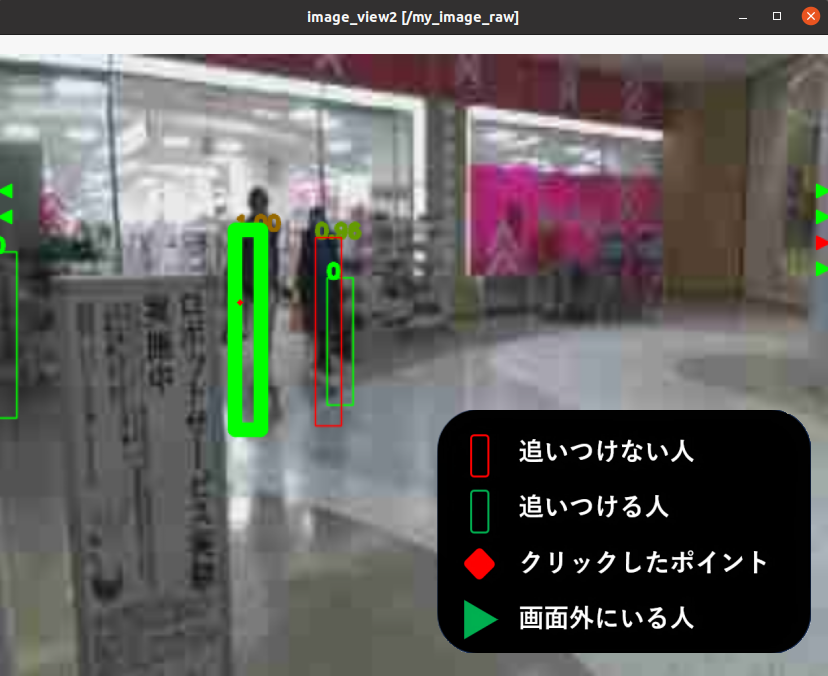
\includegraphics[width=13cm]{img/interface.png}
  \caption{操作支援インターフェース}
  \label{pic:interface}
\end{figure}
これらのシステムを用いることによって、オペレータは画面クリックのような
簡単な操作でアバターロボットを人の前まで移動させ可能な限りその人についていくことができるようになる。
これらの機能によってオペレータは歩きスマホをしている人に容易に話しかけることが可能になり、さらにその人の動きや反応に
集中できるようになる。以下では図\ref{pic:systemcompose}における各構成要素の実装について説明する。



\begin{itemize}
  \item 人位置計算 \\
  \quad 既存のソフトウェアであるhuman\_trackerを利用しており、人物の位置を取得することができる。ロボットに備わったLiDARセンサーから得られた点群データと事前に作成されたマップデータを用いており、
  点群データの内からマップデータに存在しないものを人としており、その人の位置を取得することができる。また各人に対してidが割り振られ、このidは基本人に対して唯一である。
  おおよそ1秒に5回から10回ほどの頻度で人位置と人idおよびその時刻が発行され、このデータを用いて次の速度計算が行われる。
  \item 速度・位置計算 \\
  \quad 位置の時系列データから各人idごとに速度計算と現在時点における位置計算を行う。速度計算では、まず人位置計算で得られた時刻、位置データをidごとに保存しておく。
  その後最大直近16個の時刻データと位置データを用いて、最小二乗法によって速度を計算している。
  具体的にX座標についての速度を求める場合、時刻とX座標の組を$(T_i, X_i)$とし$n(n <= 16)$個あるとする。この時その人の速度$V_x$は以下の式で求められる。
  \begin{equation}
    \label{eq: V_x}
    V_x = \frac{\sum_{i=1}^{n} (T_i - \overline{T})(X_i - \overline{X})}{\sum_{i=1}^{n} (T_i - \overline{T})^2}
  \end{equation}
  ここで$\overline{T}$は時刻の平均、$\overline{X}$はX座標の平均であり、次のようにして求められる。
  \begin{equation}
    \label{eq: average}
    \overline{T} = \frac{1}{n}\sum_{i=1}^{n} T_i, \qquad \overline{X} = \frac{1}{n}\sum_{i=1}^{n} X_i
  \end{equation}
  \quad 最大16とした理由は50等の大きい数字にすると、人の速度が変化した際に
  反応が遅くなってしまうことや計算時間の問題があり、一方で最大2個等の少ない数字にした場合は、人位置計算の結果の誤差によって速度計算の結果が大きく変動してしまったため、
  過去2秒から3秒程度で集まる16個のデータを用いることにしている。
  またhuman\_trackerからも人の速度情報を取得することができるが、式\ref{eq: V_x}
  によって求められる速度情報のほうが正確であることが確認されたため、human\_trackerから直接得られる速度情報は用いていない。 \\
  \quad またあるidの人の現在のX座標位置$P_x$はそのidの求められた速度$V_x$と現在時刻$t$を用いて、以下のように求められる。
  \begin{equation}
    \label{eq: P_x}
    P_x = \overline{X} + V_x(t - \overline{T})
  \end{equation}
  ただし、$\overline{X}, \overline{T}$は式\ref{eq: average}によって求めらるものである。
  
\quad これらによって各人の速度及び現在位置がわかる。そのデータを次のゴール計算に用いる。またhuman\_trackerの仕様上、
異なる人であっても同じidが用いられることが時々起こりうるので、その場合は過去に蓄えられたそのidに関する位置データをリセットしたのちに追加を行う。この検出は直近の位置データから大きく乖離している場合に、
異なる人であると判定を行った。
  \item 衝突計算 \\
  \quad 衝突計算では事前定数としてロボットの最大速度を、変数としてロボットの現在位置、各人の速度と位置を用いて、
各人と衝突することが可能かどうかその衝突位置を求めている。ここでの衝突は会話できる距離にいることを意味しており、具体的には
人の進行方向120cm先にロボットがいる場合を衝突としている。この値は研究\cite{mumm2011human}において、
実験の中で人がロボットにもっとも近づいた時の距離が100cmから110cm程度であったことから、両者移動していることを考慮して120cmとした。\\
\quad 具体的には以下の計算によって求めている。
人の位置を($H_x$, $H_y$)とし、ロボットの位置を($R_x$, $R_y$)とする。また人の速度を($V_{hx}$, $V_{hy}$)とし、ロボットの最大速度を$V_R$とする。また追いつくまでの時間を$t$とする。
これら用いた変数についてを表\ref{fig: variable}にまとめる。
\begin{table}[H]
  \centering
  \caption{変数・定数について}
  \label{fig: variable}
  \begin{tabular}{|c|c|c|c|}
    \hline
    人の位置 & 人の速度 & ロボットの位置 & ロボットの最大速度 \\ \hline
    $H_x$  $H_y$ & $V_{hx}$  $V_{hy}$ & $R_x$  $R_y$ & $V_R$ \\ \hline
  \end{tabular}
  
\end{table}
この時$t$秒後の人の位置は$H_x + V_{hx}t$, $H_y + V_{hy}t$であり、この位置とロボットの初期位置との距離が$V_Rt$であるので、
以下の等式が成り立つ。\begin{equation}(H_x + V_{hx}t - R_x)^{2} + (H_y + V_{hy}t - R_y)^2 = V_R^2\end{equation}
これは$t$についての二次方程式なので、tについて式\ref{eq: t}のように解くことができる。
\scriptsize
\begin{equation}
  \label{eq: t}
  \begin{split}
  t = &\frac{1}{V_{hx}^2 + V_{hy}^2}\left\{-(H_x - R_x)V_{hx} - (H_y - R_y)V_{hy} \color{white}\sqrt{(a +(c+ b))}\color{black}\right. \\
  &  \quad \pm \left. \sqrt{((H_x - R_x)V_{hx} + (H_y - R_y)V_{hy})^2 - (V_{hx}^2 + V_{hy}^2)((H_x - R_x)^2 + (H_y - R_y)^2 - V_R^2)}\right\} 
  \end{split}
\end{equation}
\normalsize
\quad この時解の内正であるものが衝突可能な時間の候補となる。
二次方程式が実数の範囲で解けない、もしくは、二つの解がともに負の値となる場合は衝突可能な時間は存在しない。また、衝突可能な時間が複数存在する場合はより小さいほうを採用する。
この解を用いて衝突可能な位置を求めることができる。実際には$H_x$, $H_y$の代わりに、人の進行方向120cm先を表す数式\ref{eq: H'}の$H'_x$, $H'_y$を用いて計算を行っている。
\begin{equation}
  \label{eq: H'}
\left\{\begin{array}{l}
H'_x = H_x + 1.2*\frac{V_{hx}}{\sqrt{{V_{hx}^2 + V_{hy}^2}}}\\
H'_y = H_y + 1.2 * \frac{V_{hy}}{\sqrt{V_{hx}^2 + V_{hy}^2}}
\end{array}\right.
\end{equation}
このようにすることによって人の進行方向120cm先と衝突できるかどうか求められる
またその際の位置$(G_x, G_y)$を式\ref{eq: t}を用いて以下のようにして求められる。
\begin{equation}
  \label{eq: G}
\left\{\begin{array}{l}
G_x = H'_x + V_{hx}t\\
G_y = H'_y + V_{hy}t
\end{array}\right.
\end{equation}
さらに人の進行方向を正面と仮定することで、人と対面することで向き$\theta$が求められる。\\
\quad このようにしてゴールポーズを求めることができた。ここでゴールポーズとは目標となる位置と向きのことである。
  \item 追従計算 \\
  \quad 人になるべくついていくためのゴールポーズを求める。そのためには、ロボットの速度ベクトルの向きは人の速度ベクトルの向きと同じになるようし、
  またその際のロボットの向きは人の向きになるようにする。よってゴールとなる位置$(G_x, G_y)$は\ref{fig: variable}で定義した変数を用いて以下のように表される。
  \begin{equation}G_x = R_x + V_{hx} \qquad G_y = R_y + V_{hy}\end{equation}
  である。また$\theta$は、$t$を$(R_x, R_y)$から$(G_x, G_y)$にたどりつくまでの時間とすると、
  $(H_x + t\,V_{hx} - G_x, H_y + t\,V_{hy} - G_y)$の偏角である。このようにして追従する際のゴールポーズが求まった。

  \item 回避計算 \\
  \quad 人とロボットの衝突をさけるため、また相手にとって不快な距離にいないようにするためのゴールポーズを求める。
  この時に進むべき方向はなるべく人から遠ざかる方向であるので、ゴールとなる位置は次の式で表される。
  \begin{equation}
    G_x = R_x + (R_x - H_x) \qquad G_y = R_y + (R_y - H_y)
  \end{equation}
  この時の向きは追従計算と同様に人の方向である。
  \item セレクター \\
  \quad セレクターは上記3つのゴールポーズから、どれを実際にゴールとするかを決定する。
  人とロボットの距離が1.2mよりも近い場合は相手にとって不快な距離にいると判断し、回避計算によって求められたゴールポーズを移動方法計算に送信する。
  人とロボットの距離が3.5mよりも近い場合は、対話可能な距離にいると判断しフォローゴールを移動方法計算に送信する。
  これは、人同士のパーソナルスペースにおいて親密でない場合の社会距離が1.2mから3.5mであることを考慮して決定した。
  3.5mよりも遠い場合には、その人と衝突可能な場合はその位置を送り不可能な場合追いつけないと判断し諦める。つまりこの時移動方法計算には何も送られない。

  \quad これらのロボットの振る舞いを説明するために、シミュレーションした結果を
  図\ref{pic:robot1}, \ref{pic:robot2}, \ref{pic:robot3}, \ref{pic:robot4}に示す。
  赤い点はロボットの位置、赤い矢印がロボットの進行方向、黒い矢印がロボットの向きを表している。
  また青い点、青い矢印は人の位置、進行方向を表しており、青い2つの円がそれぞれ3.5m、1.2mの距離を表している。
\begin{figure}[htb]
  \begin{subfigure}{0.5\textwidth}
    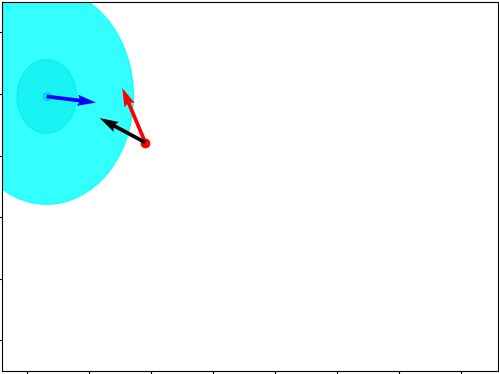
\includegraphics[width=0.95\textwidth]{img/simulation1.png}
    \caption{衝突}
    \label{pic:robot1}
  \end{subfigure}
  \begin{subfigure}{0.5\textwidth}
    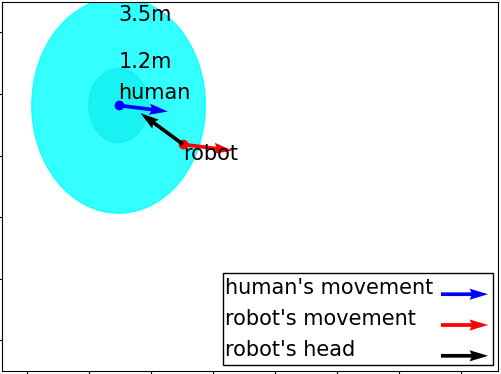
\includegraphics[width=0.95\textwidth]{img/simulation2.png}
    \caption{追従}
    \label{pic:robot2}
  \end{subfigure}
\end{figure}
\begin{figure}[htb]
  \begin{subfigure}{0.5\textwidth}
    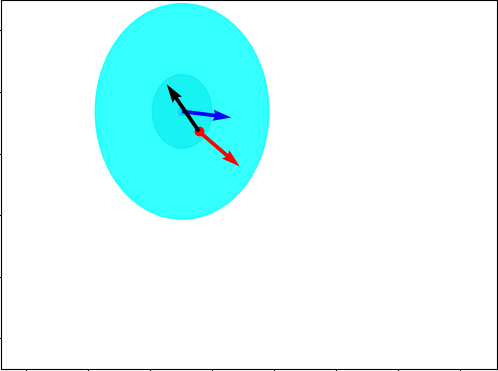
\includegraphics[width=0.95\textwidth]{img/simulation3.png}
    \caption{回避}
    \label{pic:robot3}
  \end{subfigure}
  \begin{subfigure}{0.5\textwidth}
    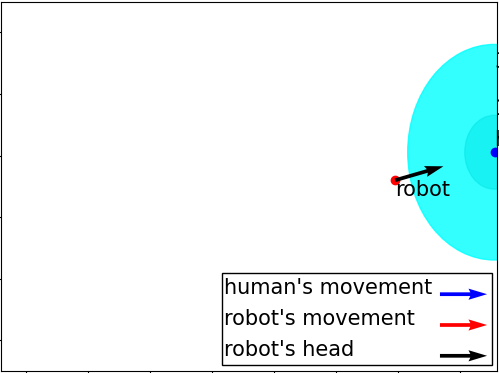
\includegraphics[width=0.95\textwidth]{img/simulation4.png}
    \caption{諦め}
    \label{pic:robot4}
  \end{subfigure}
\end{figure}
まずはじめに半径3.5mの薄青色の円に入るまでは衝突位置にむかってすすむ。その後円内では人と同じように進むが、人の速度がロボットよりも速い場合は
ロボットと人の距離が近くなりすぎる場合がある。そのような時はロボットの向きはそのままに人から遠ざかるように動く。
その後薄青色の円から出た場合は追従を諦め立ち止まる。
  \item 移動方法計算 \\
  \quad 既存のソフトウェアであり発行されたゴールポーズを目指し障害物を避けながら、ロボットに対して移動速度、回転速度についての指令を行う。

  \item インターフェース \\
  \quad ロボットに備え付けられたカメラから受け取った画像データをもとにして
  図\ref{pic:interface}のようなインターフェースを作成した。なお図\ref{pic:interface}右下に記された凡例は
  あくまでも説明のために記されたものであり、実際のインターフェースには表示されない。
  ここでは衝突計算の際の各人に対して衝突可能かどうかを用いて、
  衝突可能な人は緑枠で、不可能な人は赤枠で囲むこととしている。
  このインターフェースを用いて、オペレータは
  緑枠に囲まれた歩きスマホをしている人をクリックすることとなる。その際、ターゲットに選ばれた人を囲む枠は太くなり、オペレータは今
  だれを追跡しているかについて知ることができる。その後クリックされた人のidをゴール計算に定期的に送る。
  
  \quad また、図\ref{pic:interface}両端の赤・緑三角にてカメラに写っていない人についての情報を得ることができる。
  これはオペレータが歩きスマホをしている人を
  探す際に常に回転する必要があるという問題の解決のためであり、この機能によってオペレータは左右に人がいる場合にのみ、
  回転を行えばよい。
  
\end{itemize}
\vspace{5mm}





%\subsubsection{メディア}
%media部分では、ロボットの備え付けられたカメラのデータ、マイクのデータを取得し、インターフェースに送る。また、オペレータの発した声
%を直接そのままロボットに備え付けられたスピーカーから出力する。


\subsection{発話支援システム}


\cite{Schneider2022}では効果的な注意文言を用いることで抑止力が高まることが分かっている。
しかしオペレータがとっさにその直面する状況に対して効果的な文言を考えることは難しい。そこで
有効な注意文言の推薦を行う発話支援システムの開発によって抑止力を高めることを目指す。
図\ref{pic:speechcompose}のように注意文言データと、状況からその中で有効なものを推薦するシステムの構築
によって発話支援システムが作成可能であると考えた。以下ではそれぞれについての議論を行う。
\begin{figure}[htb]
  \centering
  \includegraphics[width=0.8\textwidth]{img/speech\_system\_compose.drawio.png}
  \caption{発話支援システムの構成案}
  \label{pic:speechcompose}
\end{figure}



なおこの発話支援は1度目の注意が無視された時に、次にかけるべき2度目の注意発話に対して行うことを想定している。
\subsubsection{有効な注意文言の検討}
\label{sec: effective}
有効な注意文言とは、\ref{sec: CDT}章で述べた中で「行動を変える」以外の解消方法に対抗するようなものである。
なぜならば、注意されてもスマホをやめない人は
注意によって生じた不快感を解消するために、\ref{sec: CDT}章で述べた解消方法の中で「行動を変える」以外のいずれか
を用いており、この解消方法に対抗するような注意によって不快感の解消を困難にし
再度不快感の解消を強いることで、「行動を変える」という解消方法をとらせる、つまり歩きスマホをやめさせることができると考えられるからである。
以下では不快感の解消はどのようにして起こるのかについて説明を行ったうえで、その後それらに対抗する具体的な文言について議論を行う。

まず多くの人が歩きスマホのことを危険だと考えており、さらに注意された際に不快感が生じることは示されている。
\cite{Schneider2022}では具体的に、以下のような過程を経ることが示されている。
\begin{itemize}
  \item[(1)] 歩きスマホをしている人も信念として、歩きスマホが危険であるという信念を持っている。
  \item[(2)] ロボットが注意を行う。
  \item[(3)] 自分の行動と信念とが矛盾していることに気付かされ不快感が生じる。
  \item[(4)] 不快感の解消のために歩きスマホをやめる。
  \item[(4')]歩きスマホをやめる以外の不快感の解消方法をとる。
  \label{item: dissonance}
\end{itemize}

歩きスマホを注意された人は
表\ref{fig: UsingPhone}のような認知を持っており、認知1と認知2の矛盾によって不快感が生じる。
\begin{table}[h]
  \centering
  \caption{歩きスマホによる不快感}
  \label{fig: UsingPhone}
  \begin{tabular}{c|c}

      認知1 & 歩きスマホは危険である  \\ \hline
      認知2 & 私は歩きスマホをしている \\ 
  \end{tabular}
\end{table}
\ref{sec: CDT}章で述べたように、注意された人は不快感を解消するためいくつかの選択肢をとることができる。
注意を受けても歩きスマホをやめなかった人は、
その中で「行動を変える」以外の選択肢をとっていると考えられる。
そこでその解消方法を無効にするような文言や、
新たに不快感を生じさせるような文言によって、再度不快感を解消する必要性を生むことで
歩きスマホをやめさせることが可能になると考えられる。

次に歩きスマホを注意された人の不快感の解消方法それぞれについて具体的に考える。
\begin{enumerate}
  \item 行動を変える \\
 行動を変えることは、歩きスマホをやめることでありこの場合これ以上注意を行う必要はない。

  \item 認知を変える \\
   認知を変えることは、表\ref{fig: UsingPhone}の認知1を「歩きスマホは危険ではない」とすることである。この認知の変更を困難にするためには、
  再度歩きスマホが危険であるような認知を追加するような文言が有効であると考えられる。例えば、
  「歩きスマホによる死亡事故例も存在します」や「歩きスマホによって他人をケガさせた場合、高額の賠償金を請求される可能性があります」
  等があげられる。
  \begin{table}[h]
    \centering
    \caption{認知の変更}
    \label{fig: AvoidDissonanceRevise}
    \begin{tabular}{c|c}
        認知1' & 歩きスマホは危険\sout{である}ではない \\ \hline
        認知2 & 私は歩きスマホをしている \\ \hline
        認知3 & 歩きスマホによる死亡事故が存在する \\
    \end{tabular}
  \end{table}
  そのような注意を受けたとき表\ref{fig: AvoidDissonanceRevise}のように認知3が追加される。
  そして、認知1'と新たに追加された認知3の矛盾により新たに不快感が生じることとなる。
  もしくは、認知1の変更が困難になる。それらの結果として、この方法での不快感の解消が難しく再び不快感の解消を試みなければならない。
  なので、この選択肢がとられた際に有効な
  注意文言は歩きスマホが危険であることを示す文言であると考えられる。

  \item 新たな認知の追加 \\
  不快感の解消のために、表\ref{fig: AvoidDissonance}の認知3や認知4が追加されることが考えられる。これらの認知は、
  認知1と認知2の矛盾を軽減させることができるため不快感の解消につながる。
  \begin{table}[h]
    \centering
    \caption{新たな認知の追加}
    \label{fig: AvoidDissonance}
    \begin{tabular}{c|c}
        認知1 & 歩きスマホは危険である \\ \hline
        認知2 & 私は歩きスマホをしている \\ \hline
        認知3 & 地図アプリを見ており、これは必要な行為である \\\hline
        認知4 & 周りに人がおらず、他人に迷惑をかけていない \\ 
    \end{tabular}
    
  \end{table}
  そこで、これらの認知の追加に対しては、認知3の追加に対して「道案内なら私がしますよ。」や認知4の追加に対して
  「そこの柱の裏から急に人が飛び出してくるかもしれません」といった文言が有効であると考えられる。
  \begin{table}[h]
    \centering
    \caption{新たな認知の追加}
    \label{fig: AvoidDissonanceBlock}
    \begin{tabular}{c|c}
        認知1 & 歩きスマホは危険である \\ \hline
        認知2 & 私は歩きスマホをしている \\ \hline
        認知3 & 地図アプリを見ており、これは必要な行為である \\
        認知3' & 道案内を目の前の人に頼むことができる \\ \hline
        認知4 & 周りに人がおらず、他人に迷惑をかけていない \\ 
        認知4' & そこの柱の裏から急に人が飛び出してくるかもしれない \\ 
    \end{tabular}
  \end{table}
  これらの
  文言は追加される認知と矛盾するものであり、図\ref{fig: AvoidDissonanceBlock}のように認知3と認知3'の矛盾を生じさせることで
  新たな不快感が生まれる、もしくは、認知3の追加を防ぐことができると予想され、結果として注意された人は再び不快感の解消を試みなければならない。
  よってこの選択肢がとられた際に有効な注意文言は、追加された認知に対して矛盾する文言であると考えられる。
  \item 矛盾の矮小化、無視 \\
  ロボットが矮小化や無視の対象となることが多い\cite{Schneider2022}。そのためこの選択肢がとられた際には、
再度ロボットを無視することが困難になるような文言が有効であると考えられる。
これは対象の外見の特徴を述べたうえで注意することによって、ロボットの矮小化を防ぐことができると考えられる。
具体例として考えられる会話の例を表\ref{dialogue: Ignore}に示した。
\begin{table}[H]
  \centering
  \caption{矮小化・無視}
  \label{dialogue: Ignore}
  \begin{tabular}{c|c}
      ロボット & 歩きスマホは危険ですので、おやめください。 \\ \hline
      人 & (無視) \\ \hline
      ロボット & そこの青いシャツを着ている方に言っています。 \\ 
  \end{tabular}
  
\end{table}
\end{enumerate}
\vspace{5mm}
以上の考察から、どのような時にどのような文言が有効であると考えられるかについてを
表\ref{fig: EffectiveWords}にまとめた。
\begin{table}[H]
  \centering
  \caption{有効な注意文言}
  \label{fig: EffectiveWords}
  \begin{tabular}{c|c|c|c}
      \multicolumn{2}{c|}{選択肢} & \multicolumn{2}{c}{有効な注意文言} \\ \hline
      \multicolumn{2}{c|}{行動を変える} & \multicolumn{2}{c}{-} \\ \hline
      \multicolumn{2}{c|}{認知を変える} & \multicolumn{2}{c}{歩きスマホは危険であることを強調するもの} \\ \hline
      \multicolumn{2}{c|}{新たな認知の追加} & \multicolumn{2}{c}{追加された認知に矛盾する文言} \\ \hline
      \multicolumn{2}{c|}{矛盾の矮小化、無視} & \multicolumn{2}{c}{対象の外見の特徴を述べた文言} \\
  \end{tabular}
\end{table}

\subsubsection{状況に応じた注意文言の推薦}

有効な注意文言の推薦のためには解消方法推定モデルの構築を行う必要がある。
なぜなら\ref{sec: effective}章で解消方法に応じた有効な注意文言について考察したが、
それらの推薦のためには、図\ref{pic:speechcompose}の注意時の状況として注意された人の解消方法を入力する必要があり、
これには認知的不協和理論に関する知識や注意された人の行動への洞察が求められる。
したがって誰にとっても有用な発話支援システムのためには、解消方法の推定をシステム側で担う必要があるからである。
そのため、実際に作るべきシステムは図\ref{pic:recommendcompose}のようになると考えられる。
\label{sec: recommend}
\begin{figure}[htb]
  \centering
  \includegraphics[width=0.8\textwidth]{img/recommend\_system\_compose.drawio.png}
  \caption{有用な発話支援システムの構成案}
  \label{pic:recommendcompose}
\end{figure}
以下では解消方法予測を行うためにモデル構築にかかわる調査を行った。


\section{ケーススタディ}
\subsection{実験目的}
\ref{sec: effective}で提案した文言による注意が有効であるかについて調べる必要がある。そのためそれら文言による注意を行い、
その後どのように感じたかについてのインタビューを行った。
また解消方法の予測モデルの構築のため、注意時の状況から注意された人の認知の状態そしてどの解消方法が取られたかについてを調べること
を目的としたケーススタディをおこなった。

\subsection{実験方法}
警備員の格好をしたアバターロボットを用い、大型のショッピングモールであるATC\footnote{https://www.atc-co.com/}の中で、歩きスマホをしている参加者に対して注意喚起を行った。また注意喚起の際に、アバターロボットを操作するためのインターフェースを用いた。
実験の様子を図\ref{fig: Experiment}に示す。
\begin{figure}[htbp]
  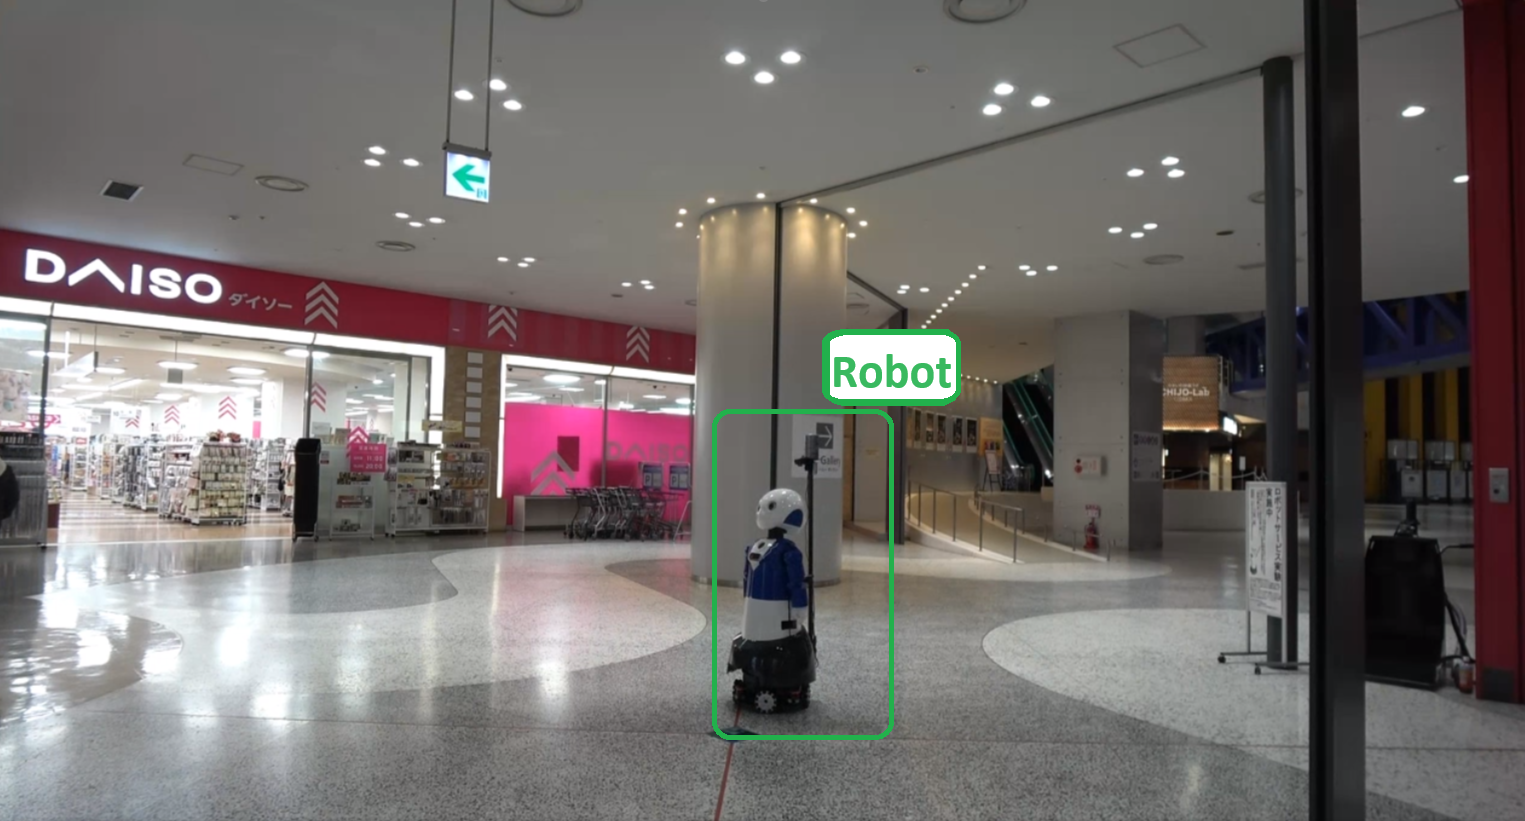
\includegraphics[width=15cm]{img/Experiment.png}
  \caption{実験環境}
  \label{fig: Experiment}
\end{figure}
中央に映るロボットが今回の実験で用いたアバターロボットで、その周囲を通った歩きスマホを
している人に対して注意喚起を行った。
\begin{figure}[h]
  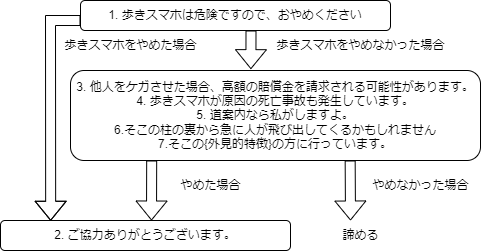
\includegraphics[width=15cm]{img/waystostop.drawio.png}
  \caption{注意文言}
  \label{fig: Strategy}
\end{figure}
用いた注意文言は図\ref{fig: Strategy}の通りであり、一度目は全員に対して
「歩きスマホは危険ですのでおやめください。」という文言を用いた。その後も歩きスマホを
やめなかった場合には、図\ref{fig: Strategy}の3,4,5,6,7の文言を用いて注意喚起を行った。
なおこの際解消方法の推定をWizard of Oz法的にオペレータが行い、それに従って注意文言を選択した。
ただしインタビューでは一回目の注意を無視するようにお願いし、
一人に対してそれぞれ一回ずつ計五回の注意を行いった。
なおいずれの場合も、二回目の注意でやめなかった時にはそれ以上の注意は行わない。

\subsection{実験参加者}
インタビューでは2人の事前に協力を頼んだ人にロボットの前で歩きスマホをしてもらい注意を行った。
またケーススタディでは5組のロボットの近くで歩きスマホをしていたATCへの来場者に対しておこなった。

\subsection{インタビュー結果}
事前に協力をお願いした二名に対して計5回注意を行い、その後どのような感想を抱いたかについてインタビューを
行った。
以下図\ref{fig: Experimentjani}, 図\ref{fig: Experimentjani2}に注意の様子を示す。
\begin{figure}[H]

  \begin{subfigure}{0.5\textwidth}
    \centering
    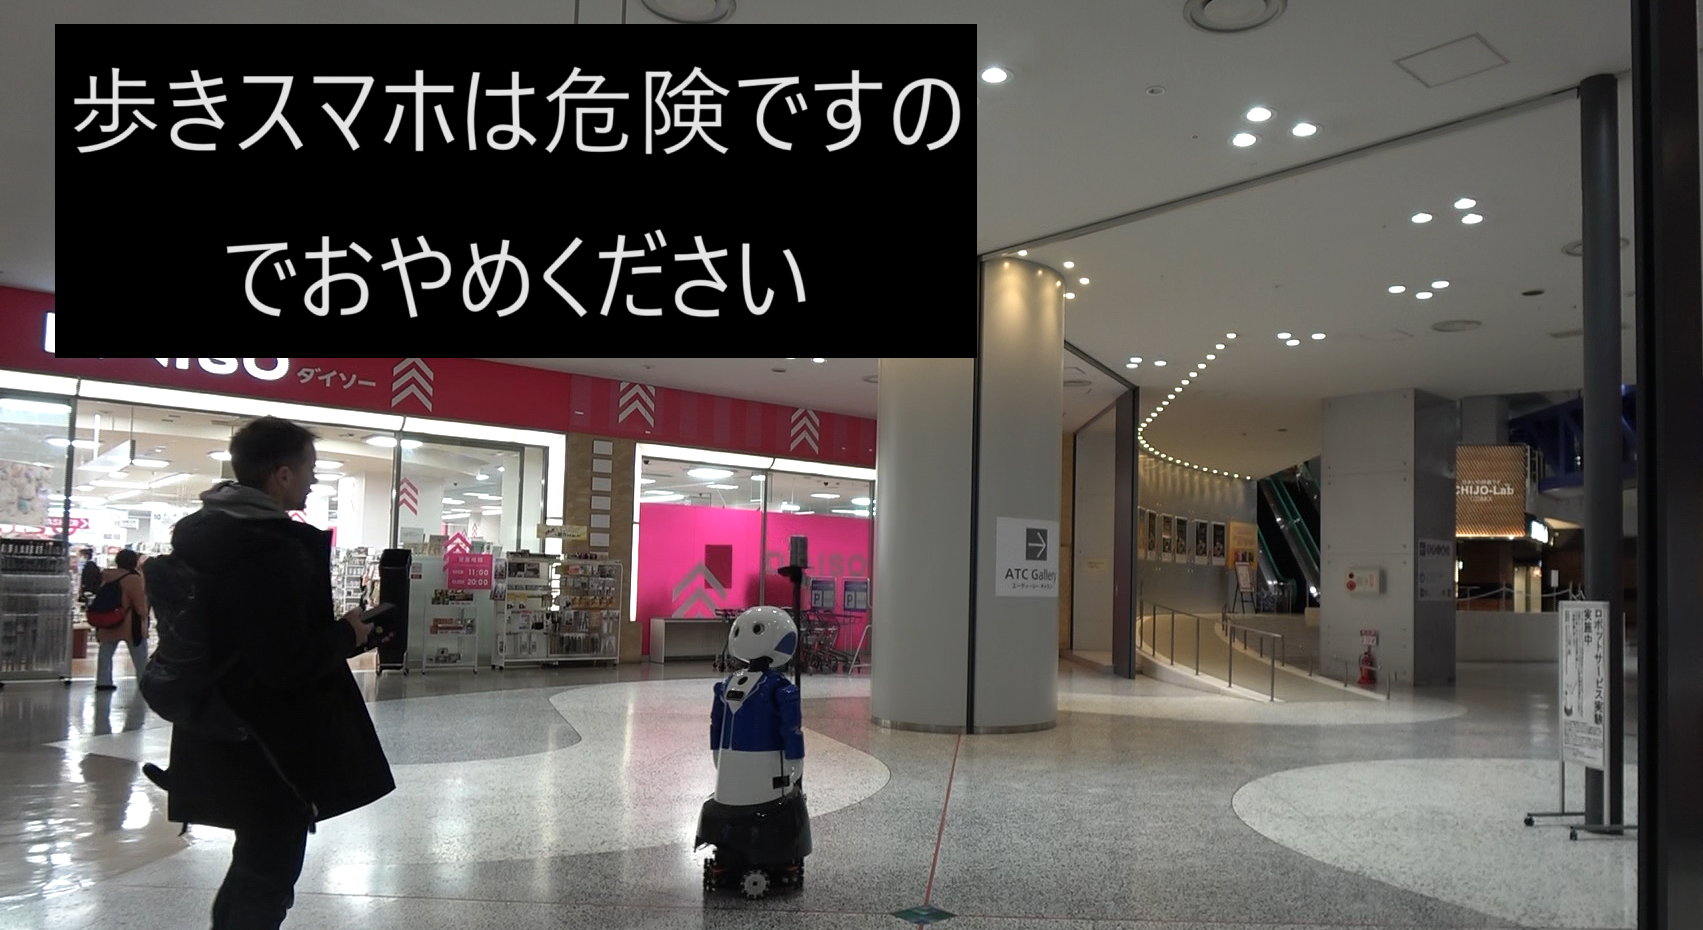
\includegraphics[width=0.95\textwidth]{img/jani2.png}
    \caption{実験の様子:一回目の注意}
    \label{fig: Experimentjani}
  \end{subfigure}
  \begin{subfigure}{0.5\textwidth}
    \centering
    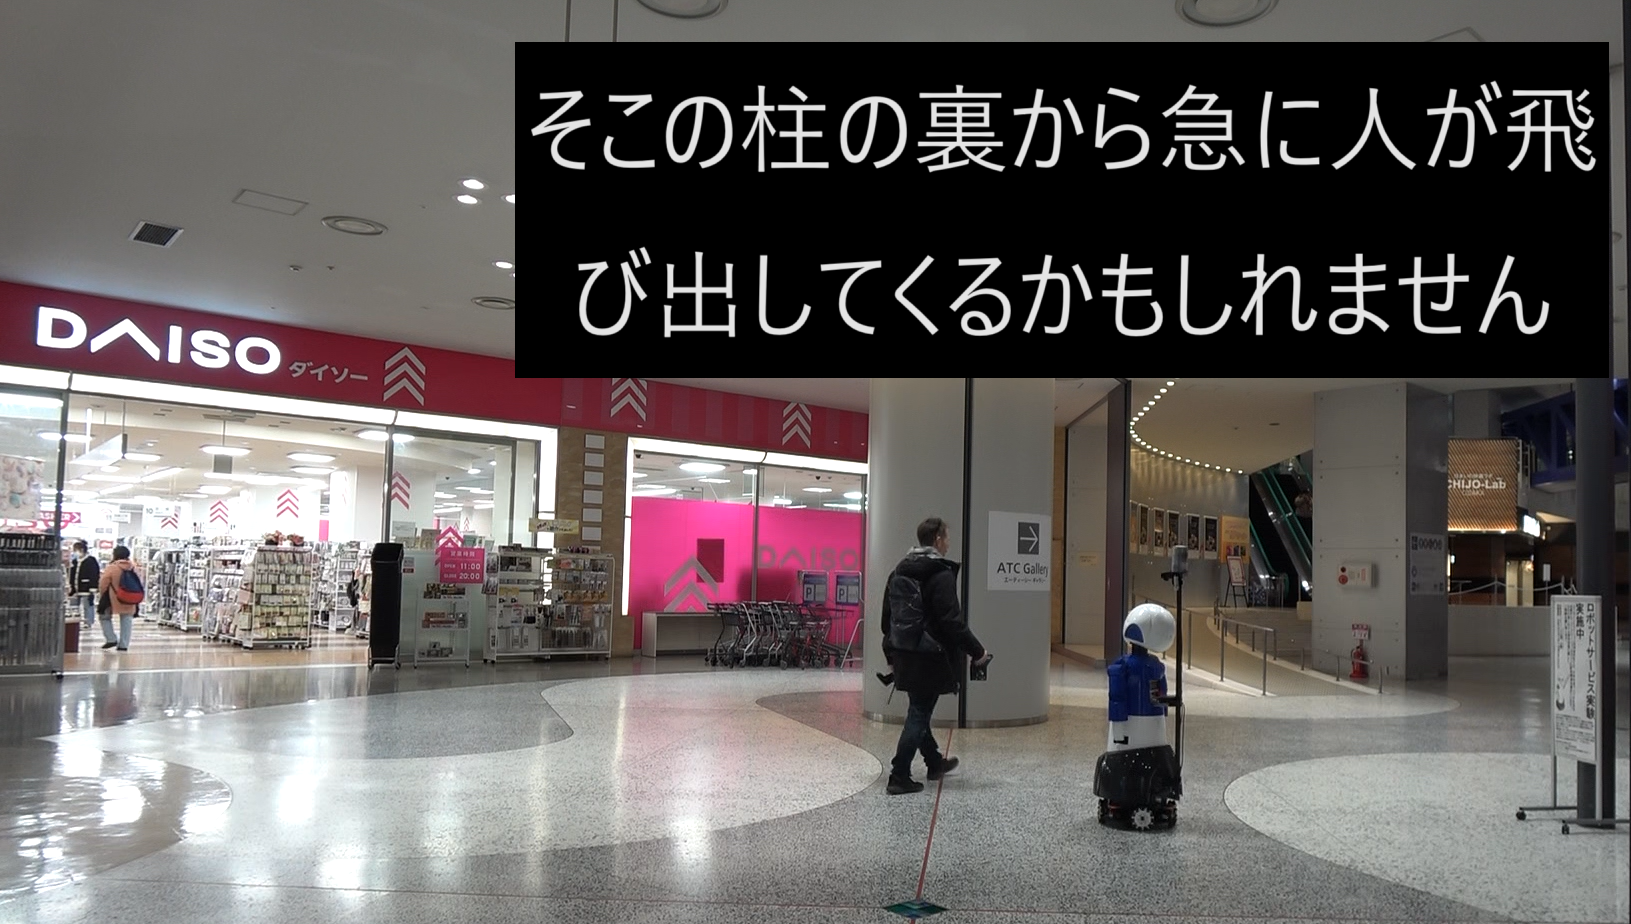
\includegraphics[width=0.95\textwidth]{img/jani3.png}
    \caption{実験の様子:二回目の注意}
    \label{fig: Experimentjani2}
  \end{subfigure}
\end{figure}
インタビューでは次のような意見が得られた。
\begin{itemize}
  \item 容姿の特徴を述べる注意文言をかけられた時に、自分が特定されていることで孤立感を感じ無視することが難しかった。
        また容姿の特徴を述べることによって周囲の人間の注目を集め、無視した際に周囲の人間からの怪訝なまなざしを向けられることも無視しづらい要因であった。
  \item 歩きスマホの危険性を強調する注意文言では、抑止力はかなり弱かった。
  \item 自分がロボットに注意されるのを目撃した他の歩きスマホをしている人は、歩くのをやめてその場で立ち止まって携帯を触っていた。
  \item ユーモアを用いるのも有効だと思った。
\end{itemize}
\subsection{ケーススタディ結果}
参加者の5組に関して注意した状況、どの解消方法が用いられたと推測され、どの注意文言を用いたか、そして結果はどうであったかについて
説明を行う。一度目の注意はいずれも「歩きスマホは危険ですのでおやめください。」という文言を用いた。
\begin{enumerate}
  \item[Case1] 男性1人でスーツを着用しており、歩行速度はかなり早めであった。一度目の注意ではこちらのほうに視線を向けることなく歩きスマホを継続した。その後、
  周囲に人がいなかったため、「周りに人がおらず、他人に迷惑をかけていない」という認知の追加によって不快感を解消していると推測し、
  「そこの柱の裏から急に人が飛び出してくるかもしれません」
  と注意した。しかし話しかけ始める時点が遅かったため、相手の後方から話すこととなり無視され歩きスマホを止めることはできなかった。
  \item[Case2] 女性2人組で片方が歩きスマホをしており、歩行速度は遅めであった。一度目の注意をおこなったところ、
  ロボットのほうを少し見たが歩きスマホを継続していた。そこで2人組であり片方の1人のみが歩きスマホをしていることから、
  地図アプリを使用していると考え、「地図アプリを見ており、これは必要な行為である」という認知の追加によって不快感を解消していると推測した。
  そして「道案内なら私がしますよ」と話すと、「駅の方に行きたいです」と返答があったためその方向を指し示した。その後歩きスマホをやめたがスマホは手に持ったままであった。
  なおこの時、彼女らが向かっていた方向は駅の方向ではなく反対側であった。
  \item[Case3] 男性1人で平均的な速度であった。一度目の注意に対して、英語で「私は中国人なので中国語で話して」と返答があったため、
  中国語を話せる人にオペレータを代わってもらい、中国語で注意を行ったところロボットを凝視したのちに歩きスマホをやめ歩行を再開したが、
  その後しばらくの間もロボットを見ていた。
  \item[Case4] 男性1人で歩行速度はかなり遅めであった。1度目の注意でこちらに少し目を向け歩きスマホをやめ歩行速度を速めた。そのため
  2度目の注意は行わなかったが、実際はしばらくしたのちに歩きスマホを再開していたが、オペレータはそのことに気づかなかった。
  \item[Case5] 男女複数名のグループで全員スーツを着用しており、そのうち1人の女性が歩きスマホをしていた。グループ全体の歩行速度は平均的であった。
  一度目の注意で歩きスマホをやめ、それ以上の注意は行わなかった。その後グループの何人かがロボットのほうを見て
  ロボットについて話をしていた。
\end{enumerate}
特にCase2の様子を図\ref{fig: Case2}に示す。
\begin{figure}[H]
  \centering
  \begin{subfigure}{0.33\textwidth}
    \centering
    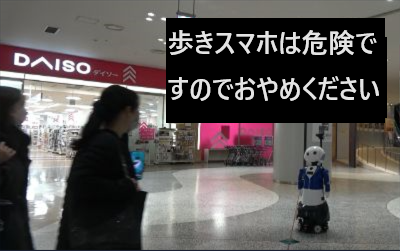
\includegraphics[width=0.95\textwidth]{img/Case2-1.png}
    \caption{一度目の注意}
    \label{fig: Case2_1}
  \end{subfigure}
  \begin{subfigure}{0.33\textwidth}
    \centering
    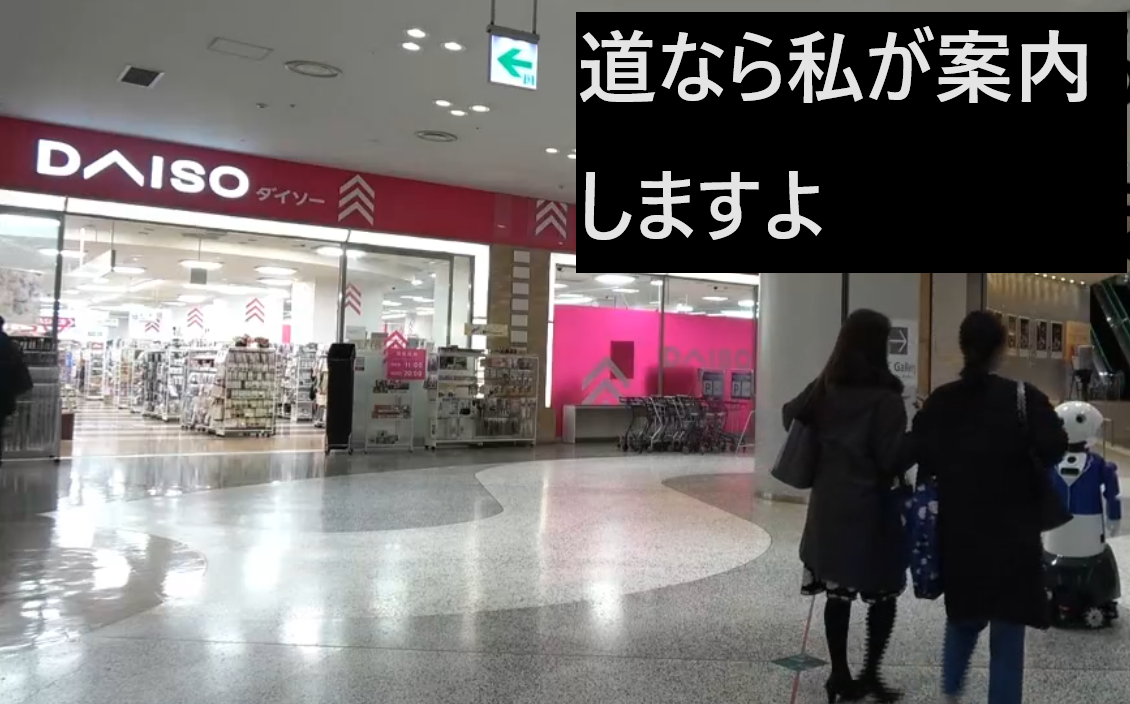
\includegraphics[width=0.95\textwidth]{img/Case2-2.png}
    \caption{二度目の注意}
    \label{fig: Case2_2}
  \end{subfigure}
  \begin{subfigure}{0.33\textwidth}
    \centering
    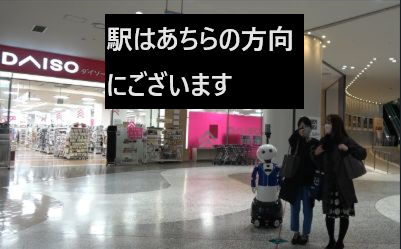
\includegraphics[width=0.95\textwidth]{img/Case2-3.png}
    \caption{駅への案内}
    \label{fig: Case2_3}
  \end{subfigure}
  \label{fig: Case2}
\end{figure}

\subsection{実験結果の考察}
実験での観察から解消方法の識別に重要な属性として、周囲の状況、歩行速度、恰好、
グループの人数、注意された際の反応があると考えられる。例えばスーツを着用している人は普段からATCを利用している人が多いと考えられるため、地図アプリを見ている可能性は低い。
しかしCase2のように歩行速度が遅い場合、地図アプリを利用している可能性が高く「道案内なら私がしますよ」という文言が有効になる。

実際にそれらの属性の値によってそれぞれどのような解消方法が用いられたかについて考察が可能である。
Case1では一度もロボットへの反応を示すことなく歩きスマホを継続しており、
一方Case4では一度ロボットへ反応を示し歩きスマホをやめたのちに再開していた。
このことから、実験時Case1では「認知の追加」、Case4では「行動の変化」によって不快感を解消していると推測したが、
実際はそれぞれ「無視、矮小化」、「認知の追加」によって不快感を解消していたため注意がうまくいかなかったと考えられる。
なぜなら「無視、矮小化」では実際に認知になにも変化は起きていないため、注意された際即座に不快感の解消を行うことができる。
一方で「認知の追加」の場合、なにかしらの認知を追加する必要があるため解消までに時間がかかる。
そこで合理的な認知を追加されるまで、歩きスマホをやめることによって解消を行い、その後認知の追加によって解消を行い再び歩きスマホを再開したと予想される。

また解消方法に基づいた注意文言によって歩きスマホをやめさせることが期待できる。
Case2では行きたい方向の逆方向に歩いていたことから、地図アプリを使用していたと考えられる。
そのためCase2は解消方法をうまく推測でき、実際にそれに対抗する文言によって歩きスマホを止めることができた例となる。
さらにCase3では、その発言内容から「たかがロボットが中国語話せないでしょ」とロボットを矮小化していると予測される。
その中で中国語で注意したことで、実験時は解消方法について推測できていなかったが、結果として矮小化を防ぐことができたため歩きスマホを
やめさせることができたと考えられる。

アンケートからは周囲の人から注目されている時には無視することが難しいという意見が得られた。
これは不快感の解消のために歩きスマホをやめたのではなく、周囲の人々の同調圧力から歩きスマホをやめたと考えられる。
また歩きスマホの危険性を強調する文言の抑止力が弱いという意見が得られたが、
これは無視するようにお願いしているため「実験のために歩きスマホをしている」という認知が追加されており、
不快感が生じなかったことが原因と考えられる。

これらの結果から解消方法に対抗する文言によって抑止力の向上が見込めることと、
周囲の状況、歩行速度、恰好、グループの人数、注意された際の反応がそれら識別に重要であることが分かった。
ほかにもユーモアや同調圧力を用いた戦略が有効であることが示唆された。

\section{今後の課題}
今回解消方法の判断において重要であろうと考えられる属性をいくつか見つけることができたが、
それらの属性の値によってどのような解消方法がとられたかを明確にすることはできていない。
さらに追加される認知や、無視、矮小化の対象には実験で想定した以外の様々なものが考えられる。
そのため発話支援システムの開発のために、今後実験によってどのような解消方法が考えられるのかについての
研究、および上記の属性の値から解消方法を予測するようなモデルを構築することが必要である。
また不協和を利用した戦略以外にも、アンケートからは同調圧力を用いた戦略を取り入れたシステムも考えられる。


移動に関して今回のシステムでは単純に歩きスマホをしている人に一直線に近づくというものであったが、
\cite{Mizumaru2019}のように工夫した近づき方を行うことで、より注意をひきつけ抑止力の向上につながるはずである。
\section{まとめ}
本研究ではアバターロボット警備員業務の中で歩きスマホを注意する際に、問題となる移動操作の困難性と
抑止力の欠如を解決するためにオペレータを支援するシステムの実装を行った。

第一に、コントローラーを用いて歩きスマホをしている人に近づき、継続的にその人の方向を向いているという操作が
困難であるという移動操作に関する問題を解決するインターフェースおよびシステムの構築を行った。
これにより、オペレータはカメラ映像上で人をクリックするだけで、その人に適切に追従することができるようになった。

ロボットに注意されたときにたかがロボットと侮られ無視されやすいことに加えて、
オペレータが効果的な注意文言をとっさに考え付くことが難しいことから生じる抑止力の欠如を
効果的な注意文言を推薦するような発話支援システムを作成することで解決できると考えた。

そこで第二に発話支援システムの構築に当たり、まず効果的な文言がどのようなものであるかについて認知的不協和理論に基づき考察を行い、
注意によって生じた不快感は行動を変える以外の方法によっても解消できることに着目し、それらの解消方法に対抗しもう一度不快感の解消をせまるような文言が効果的であると結論づけた。
しかし今のままでは推薦のために注意された人がとったであろう解消方法を推測する必要があり、
これには認知的不協和理論に関する知識や注意された人の行動への洞察が求められる。
そのためすべての人に対して有用な発話支援システムのためには、解消方法の推定をシステムが担う必要がある。

そこで第三に、解消方法の識別に必要な情報を得るための実験を行った。その結果として、
いくつかの属性が解消方法の識別に重要であることや提案したもの以外の有効な注意文言が考えられることがわかった。
将来課題として
これらの属性を用いた解消方法の予測モデルの構築を行い、それを用い有効な注意文言の提示を行うシステムの構築や
その他の戦略を取り入れることがあげられる。

%=====================================================================================
\acknowledgments %章を付けずにタイトル表示
本研究を行うにあたりご指導頂いた指導教員の神田崇行教授と Jani Even
特定講師、今回の研究の予備実験を手伝ってくださった
友人たち、本論文の執筆にあたり多くのご助言をいただいた先輩方、そして実験を行うに当たって協力頂いたATRの方々と実験に協力してくださったATCの来客者の方々
に深い感謝の気持ちとお礼を申し上げ
ます。

%=====================================================================================
\nocite{*}
\bibliography{citation} %bibtexファイルの読み込み
\bibliographystyle{kuisunsrt} %本文に\cite{}を入れることで,参考文献表示

\end{document}